\chapter{Species diversification model}
{\color{gray} \begin{fquote}[Finman's Law]  Nobody wants to read anyone else's formulas. \end{fquote} }



For this chapter we will use the following notation:

%\begin{center}
%{\Large \bf Notation}
%\end{center}


\begin{description}[leftmargin=!,labelwidth=\widthof{\bfseries The longest label}]
%\item[$T$] : Time of speciation or extinction (Random Variable).
\item[$t_i$] : Branching time $i$.
\item[$n_i$] : Number of species at time $t_i$.
\item[$m$] : Number of covariates
\item[$S_i = \{ s_{i,1},...,s_{i,n_i}\}$] : Set of extant species at time $t_i$.
\item[$\lambda_{i,j}$] : Speciation rate for specie $s_{i,j}$ (at time $t_i$).
\item[$\mu_{i,j}$] : Extinction rate for specie $s_{i,j}$ (at time $t_i$).
\item[$\mathfrak{s}_i$] : Species which got speciation or extinction at time $t_i$ (note that $\mathfrak{s}_i \in S_i$ as well). 
\item[$\mathfrak{x}_1$] : Binary value; $\mathfrak{x}_i =$ "extinction" ($0$) if an extinction occurs at time $t_i$ and $\mathfrak{x}_i =$ "speciation" ($1$) if an speciation occurs at time $t_i$. 
%\item[$\pi_i$] : $\mathfrak{x}_i$ rate of specie $\mathfrak{s}_i$.  
\item[$\rho_i$] : $\mathfrak{x}_i$ rate for specie $\mathfrak{s}_i$.
\item[$x_{i,j,k}$] : $k$-covariate of the specie $j$ at time $t_i$.
\end{description}

\vspace{1cm}
\newpage
\section{Process}
We start defining the following sets: 

$$\mathcal{T} = \{t_1,...,t_p\}$$
$$\mathfrak{S} = \{\mathfrak{s}_1,...,\mathfrak{s}_p\}$$
$$\mathfrak{X} = \{ \mathfrak{x}_1, ..., \mathfrak{x}_n \} $$

The phylogenetic tree is mathematically determined by

\begin{itemize}
	\item A set of branching times $\mathcal{T}$.
	\item The topology  $\Upsilon = \{ \mathfrak{S}, \mathfrak{X} \}$.   
\end{itemize}


It is natural to assume \cite{Phyl} that the time needed for the species $s_{i,j}$ to get speciated follows an exponential distribution with parameter $\lambda_{i,j}$ and the time, of the same species, needed to get extinct follows an exponential distribution with parameter $\mu_{i,j}$. Thus, the waiting time $T_i$, defined as the minimum time, among all species, to have an speciation or extinction, also follows an exponential distribution  

	$$ P(T_i = t) = \sigma_i e^{-\sigma_i t} $$ 
	
where $\sigma_i$ is the sum of all speciation and extinction rates of extant species at time $t_i$\footnote{Note that if $X_i \sim exp(p_i)$, then $X = \min\{X_i,...,X_n\}\sim exp(\sum p_i)$. For details see \cite{casella}}. That is $\sigma_i = \sum_{j=1}^{n_i} \lambda_{i,j} +\mu_{i,j} $. \\

Moreover, given the waiting time $t_i$, the probability of speciation of the species $s_{i,j}$ is $\frac{\lambda_{i,j}}{\sigma_i}$ and the probability of extinction of the same species is $\frac{\mu_{i,j}}{\sigma_i}$.\\

		
 Then, the general version for the likelihood function of the phylogenetic tree is
 
 		\begin{equation} L( Y | \Theta) = \displaystyle\prod_{i=1}^p \sigma_i e^{-\sigma_i t_i} \frac{\rho_{i}}{\sigma_i}  
 		\label{llik}
 		\end{equation}
 		
Note that
 
\begin{itemize}
 	
 	\item $\lambda$ and $\mu$ are non-constants but functions of explanatory variables, which includes traits values, environmental phenomena, location, diversity of species or time, which makes the model fairly flexible. 
 	\item The probability of $\Upsilon$ follows a Multinomial distribution $M(n | \lambda,\mu)$ with $n=1$. However we could easily use $n > 1$ which would consider the case of multiple speciation \cite{multi}.
 	 \end{itemize}
 	 
 	

 	 
 By tacking partial derivatives equal to zero an analytical solution for \ref{llik} in the case of constant rates can be easily calculated; however, as mentioned on the previous chapter, our general (scientific) interest is to find insights of several ecological factors which could have a potential impact on the evolutionary processes of species, thus, the diversification rates are actually functions of explanatory variables
 
 %% why linear?

 $$ \lambda_{i,j} = f(\langle x_{i,j,\cdot}, \beta_1 \rangle ) $$
 $$ \mu_{i,j} = f(\langle x_{i,j,\cdot}, \beta_2 \rangle ) $$

where $\beta_1$, $\beta_2$ are $m$-dimensional vectors of parameters and $x_{i,j,\cdot}$ are $m$-dimensional vectors of ecological data (explanatory variables). $\langle \cdot, \cdot \rangle $ represents the inner product of two vectors.  \\


%On this project we will start studding the cases 
%
%\begin{itemize}
%	\item $f(x) = x$
%	\item $f(x) = e^x $
%\end{itemize}
%
%However this can be extended to any other possible biological relationship. \\
   
 For non-constant rates there is no analytical solution. We used standard optimization algorithms \cite{Bertsekas} to minimize the likelihood for three different covariates models, however, those methods are not stable. \\
 
   
 
 \section{Estimation}
 
 We are seeking for an stable and flexible method for parameter estimation and model selection. With this purpose, and considering our particular likelihood function, which has parameters which are in turn function of explanatory variables, it worth to introduce a well known statistical kind of models, the Generalized Linear Models.
 
\subsection{Generalized Linear Models}

 The unity of many statistical methods was demonstrated by Nelder and Wedderburn \cite{nelder} using the idea of the Generalized Linear Model (GLM). We present here the general set up for the Generalized Linear Model, specially applied to our research case. For a detailed study of GLM theory we refer the reader to \cite{Dobson2008} or \cite{mccullagp.j.a.nelder1989}.\\ 

Let $Y_1, Y_2, ..., Y_n$ be independent random variables, from the exponential family \footnote{For details regarding to the required mathematical assumptions concerning the exponential family of distributions we refer the reader to \cite{casella}}, and $X$ non-random matrix of explanatory variables or covariates \footnote{In our case, we are interested on potential effects of ecology factors on evolutionary processes. Then, different traits of species, climate, geographic characteristics, time and diversity of species are possible covariates of our random variable $Y$}. In general, to specify a GLM we need 

\begin{itemize}
	\item The probability distribution of $Y_i$.
	\item Equation linking the expected value of $Y_i$ with a linear combination of the explanatory variables.
	
\end{itemize} 


On this way we split the model on a random component and a systematic component, where the random component specifies the distribution of $Y_i$ and the systematic component specifies the way in which the explanatory variables comes into the model. Note that, unlike the current methods mentioned on previous chapter, we are not directly interested on estimate speciation and extinction rates itself, but we want to estimates the critical parameters which controls the underlining processes on ecological evolution. The diversification rates are functions of these parameters. 

Thus, we choose a function $g$ such that 

		$$ g(E(Y)) = \eta_i = \langle \bf{x_i}, \bf{\beta} \rangle $$
		 
where: 

\begin{itemize}

	\item $g$ is a monotone, differentiable function called the \emph{link function}.
	
	\item The vector $\bf{x}_i$ is a $m \times 1$ vector of explanatory variables.
	
	\item $\bf{\beta}$ is a $m \times 1$ vector of parameters.
	

\end{itemize}

The vector $\bf{x_i}^T$ is the $i$th row of the design matrix $\bf{X}$.\\

Note that the inference of $\beta$ is crucial in the ecological sense, as those are the indicators of relationship of ecological factors and evolutionary processes. On this project we focus our attention on the development of an efficient framework able to capture this relationship; $g(\cdot)$ expresses the relationship of the covariates as a function of $E[Y]$. \\


Summarizing, a generalized linear model has three components:

\begin{enumerate}
	\item Response variables $Y_1,...,Y_n$ from the exponential family.
	\item A set of parameters $\bf{\beta}$ and explanatory variables $\bf{X}$.
	\item monotone link function $g$ such that 	
		$$ g(E(Y_i))=\langle \bf{x}_i, \bf{\beta} \rangle $$
\end{enumerate}

%\newpage

\subsubsection{Iterative Re-Weighed Least Squares algorithm (IRWLS)}

For the estimation of parameters we use the IRWLS method [Charnes et al. 1976], which is based on the the method of scoring which in turn is based on the Newton-Raphson formula, \\

Basically, the method has the following structure:\\

 \vspace{1cm}
\fbox{%
    \parbox{12cm}{%
\begin{itemize}
	\item[i.] Obtain an initial estimate $\bf{\beta}$,
	\item[ii.] replace $f(y_i,\beta)$ with a Taylor series approximation,
	\item[iii.] evaluate all expressions that involve $\beta$ at the current estimate,
	\item[iv.]	 solve the resulting system of equations
	\item[v.] actualize the new $\beta$ and repeat (ii)-(v) until $\{ \beta^k \}$ converges.
	
\end{itemize}
}
}


.\\
\vspace{1cm}

Thus, the general formulation in the GLM context has the form,

\begin{equation} \bf{\beta}^{(m)} =  \bf{\beta}^{(m+1)} + [\mathcal{J}^{(m-1)}]^{-1}U^{(m-1)} 
\label{iterGLM}
\end{equation}

or 

\begin{equation} \mathcal{J}^{(m-1)}\bf{\beta}^{(m)} =  \mathcal{J}^{(m-1)}\bf{\beta}^{(m+1)} + U^{(m-1)} 
\label{iterGLM2}
\end{equation}


where $\bf{\beta}^{(m)}$ is the vector of estimates of the parameters $\beta_1, ... , \beta_l $ at the $m$th iteration, $[\mathbb{J}^{(m-1)}]^{-1}$ is the inverse of the information matrix and $U^{(m-1)}$ is the score function evaluated on $\bf{\beta}^{(m-1)}$. \\

Thus, we can re-write the information matrix as 

$$ \mathcal{J} = X^TWX $$

where $W$ is the diagonal matrix with elements

$$ w_{ii} = \frac{1}{Var(Y_i)}\left( \frac{\partial E(Y_i)}{\partial \eta_i} \right)^2 $$

and the expression on the right-hand side of \ref{iterGLM2} can be written as 

$$X^TW\bf{z}$$

where $\bf{z}$ has elements

$$ z_i = \langle \bf{x_i},\beta \rangle + (y_i - E(Y_i)) \left( \frac{\partial \eta_i}{\partial E(Y_i)} \right) $$

with $E(Y_i)$ and $\frac{\partial \eta_i}{\partial E(Y_i)}$ are evaluated at $\bf{\beta}^{(m-1)}$. 

Hence the iterative equation \ref{iterGLM} can be written as
%
$$X^TWX\bf{\beta}^{(m)}=X^TW\bf{z}$$
%

This is the same form as the normal equations for a linear model obtained by weighed least squares, except that it has to be solved iteratively because, in general, the components of the equation depends on $\beta$. 

\subsection{Maximun GLM likelihood for phylogenetic trees}

The implementation of the previous ideas on the phylogenetic tree has mainly two simultaneous GLM, the branching times (Br) GLM and the Topology (To) GLM. Thus, we re-write equation \ref{llik} considering both parts
 
 		\begin{equation} L( Y | \Theta) = \displaystyle\prod_{i=1}^p \displaystyle\underbrace{\sigma_i e^{-\sigma_i t_i}}_{Bt} \displaystyle\underbrace{\rho_i / \sigma_i}_{To}  
 		\label{llik2}
 		\end{equation}
 		
and we are looking for the log-likelihood function

$$ l(\beta) = l^{Bt}(\beta) + l^{To}(\beta) $$
 		
 Our aim is to find the MLE of \ref{llik}, that is
 
 
 $$ \hat{\beta} = \displaystyle\argmax_{\beta} l(\beta) = \displaystyle\argmax_{\beta} l^{Bt}(\beta) + l^B(\beta)$$ 
 
 
Then, for the whole phylogeny we consider 

$$X^TWX = X^{Bt}W^{Bt}X^{Bt} + X^{To}W^{To}X^{To} $$
 
thus, our iterative procedure corresponds to 
\begin{equation}
  X^T W X\beta^{(m)}=X^TW\bf{z}
  \label{iter}
\end{equation}
 where
 
 \[
X=
  \begin{bmatrix}
    X^{Bt} \\
   X^{To}
  \end{bmatrix},
\]

\[
W =
  \begin{bmatrix}
    W^{Bt}   &  0 \\
    0 &  W^{To} 
  \end{bmatrix}
\]
and 
  \[
Z=
  \begin{bmatrix}
    Z^{Bt} \\
   Z^{To}
  \end{bmatrix}
\]


thus, to performs the MLE minimization we need the formulation of $$X^{Br}, W^{Br}, Z^{Br}, X^{To}, W^{To}, Z^{To}.$$  

\subsubsection*{The branching times (Bt)}
	
As mentioned before, $T_i$ follows an exponential distribution 
	
	$$ P(T_i = t_i) = \sigma_i e^{-\sigma t_i} $$
	
thus 

\begin{equation}
E(T_i) = \frac{1}{\sigma_i}  \text{ and } Var(T_i) = \frac{1}{\sigma_i^2}
\label{espvar1}
\end{equation}


By other side, we have 

%$$ \sigma_i = \displaystyle\sum_{j=1}^{n_j} \rho_{i,j} =  \displaystyle\sum_{j=1}^{n_j} \langle x_{i,j}, \beta \rangle = \langle \sum_j x_{i,j} , \beta \rangle = \langle \bf{x}_i , \beta \rangle $$

\begin{align*}
\sigma_i &= \displaystyle\sum_{j=1}^{n_i} \lambda_{i,j} + \mu_{i,j} \\
	     &= \displaystyle\sum_{j=1}^{n_i} \langle x_{i,j,\cdot}, \beta_1 \rangle + 				\langle x_{i,j,\cdot}, \beta_2 \rangle \\
	     &= \langle \sum_j x_{i,j,\cdot}, \beta_1 + \beta_2 \rangle \\ 
	     &= \left\langle \bf{x}_i^{Bt} , \beta^{Bt} \right\rangle 
\label{linear}
\end{align*}


%
then, by \ref{espvar1}, the equation above, and following the GLM procedure, we get the link function $g(x) = 1/x$. \\

we use this to calculate the matrix $W$, 

$$ w_{ii}^{To} = \frac{1}{Var(T_i)}\left( \frac{\partial E(T_i)}{\partial \eta_i} \right)^2 $$

where, $Var(T_i)$ is given by \ref{espvar1} and 

$$ \frac{\partial E(T_i)}{\partial \eta_i} = \frac{\partial g^{-1}(\eta_i)}{\partial \eta_i} = \frac{\partial \frac{1}{\eta_i}}{\partial \eta_i} = -\frac{1}{\eta_i^2} = -\frac{1}{\left\langle \bf{x}_i , \bf{\beta} \right\rangle ^2} $$ 

Then, $$w_{ii} = 1/\langle \bf{x}_i , \beta \rangle ^2, \forall i$$
Thus, 

\[
W^{Bt}=
  \begin{bmatrix}
    1/\sigma_1     &      0 & \cdots &  0 \\
     0     &     1/\sigma_2 & \ddots &  0 \\
    \vdots & \ddots & \ddots  & 0 \\
     0     &      0 & 0 &  1/\sigma_p 
  \end{bmatrix}
\]

%Following the GLM procedure, let $g(x)$ be a real function such that 
%$$ g(E(T_i)) = g(\frac{1}{\sigma_i})  = \langle \bf{x}_i , \beta \rangle  $$   

%then, $g(x) = 1/x$ 


Moreover, 

$$
 z_i^{Bt}  = \langle {\bf x_i},\beta \rangle + (t_i - E(T_i)) \left( \frac{\partial \eta_i}{\partial E(T_i)} \right)  = \sigma_i(2-t_i\sigma_i)
$$



Then, we could compute the IRWLS iterations for the exponential distribution case


$$(X^{Bt})^TW^{Bt}X^{Bt}\bf{b}^{(m)}=(X^{Bt})^TW^{Bt}\bf{z}^{Bt}$$

where 

\[
X^Bt=
  \begin{bmatrix}
    \sum_j x_{1,j,1}     &   \sum_j x_{1,j,2} & \cdots &  \sum_j x_{1,j,m} \\
    \sum_j x_{2,j,1}     &   \sum_j x_{2,j,2} & \ddots &  \sum_j x_{2,j,m} \\
    \vdots & \ddots & \ddots  & \vdots \\
     \sum_j x_{p,j,1}     &      \sum_j x_{p,j,2} & \cdots &  \sum_j x_{p,j,m} 
  \end{bmatrix}
\]

with $x_{i,j,k}$ is the $k$-covariate for the specie $j$ at time $t_i$. \\



%This is half of our log-likelihood function, let's check the multinomial part


\subsubsection*{The topology}


 As described previously the topology $\Upsilon_i$ follows a multinomial distribution \\ $MN(1,\lambda_1,\mu_1,\lambda_2,\mu_2,...,\lambda_{n_i},\mu_{n_i})$, \\
 
 
 for convenience, we define $\pi_i=\frac{\rho_i}{\sigma_i}$, where $\rho_i$ is the $\mathfrak{x}_i$ rate of the specie $\mathfrak{s}_i$ \footnote{Note that $\mathfrak{x}_i$ is a string corresponding to "speciation" or "extinction", please see the notation section for details.}. In other words, $\pi_i$ is the probability that the specie $\mathfrak{s}_i$ evolves at time $t_i$ as had happened.
 
 Then, we define the Bernoulli distributed random variable $Z_i \sim B(\pi_i) $, \\
 
note that 

$$ l^{To}=L(Z_i|\pi) = \displaystyle\prod_{i=1}^n \pi_i $$

and $E[Z_i] = \pi_i$,        $Var(Z_i) = \pi_1(1-\pi_i)$
	
then, we can work with $Z_i$ instead of $\Upsilon_i$ as they have same Likelihood function. 

we can $\pi_i$ this as 

$$ \pi_i = \frac{\eta_i}{\eta_i + c_i} $$ 

where $\eta_i = \langle x_{i,\mathfrak{s}_i},\beta \rangle $ and $c_i = \langle \displaystyle\sum_{j\neq \mathfrak{s}_i}^{n_i} x_{i,j}, \beta \rangle $. Thus, 

$$ \eta_i^{To} \frac{1}{c_i} = \frac{\pi_i}{1-\pi_i} $$ 

and 
 $$g(\pi_i) = \frac{\pi_i}{1-\pi_i} $$ 
	
then, 	
	% caminar por las calles de paris me recuerda la cuidad de mi amor <3... por el olor a meao nomas si, por que valpo es infinitamente mas maravilloso que paris :).
	\[
X^{To}=
  \begin{bmatrix}
 	x_{1,\mathfrak{s_1},1} & x_{1 , \mathfrak{s}_1 , 2} & \cdots & x_{1,\mathfrak{s}_2,m} \\
 	x_{2,\mathfrak{s_2},1} & x_{2,\mathfrak{s}_2,2} & \cdots & x_{2,\mathfrak{s}_2,m} \\
 	\vdots & \ddots & \cdots & \vdots \\
 	x_{p,\mathfrak{s_p},1} & x_{p,\mathfrak{s}_p,2} & \cdots & x_{p,\mathfrak{s}_p,m} \\
  \end{bmatrix}
\]


$$w_{ii}^{To} = \frac{1}{\pi_i(1-\pi_i)}\frac{c_i^2}{(\eta_i+c_i)^4} = c_i\pi_i^2$$

and

\[
W^{To}=
  \begin{bmatrix}
    c_1\pi_1^2     &      0 & \cdots &  0 \\
     0     &    c_2\pi_2^2 & \ddots &  0 \\
    \vdots & \ddots & \ddots  & 0 \\
     0     &      0 & 0 & c_p\pi_p^2
  \end{bmatrix}
\]

moreover, 

$$ z_i^{To} = \displaystyle\sum_{k=1}^m x_{i,\mathfrak{s}_i,k} \beta_k + \frac{\pi_ic_i^2}{(1-\pi_i)^3} $$
	
	
then, $Z^{To} = [z_1^{To},...,z_p^{To}]^T$.


 \subsubsection*{The phylogenetic tree (branching times + topology)}
 
 Finally, we have $$X^{Br}, W^{Br}, Z^{Br}, X^{To}, W^{To}, Z^{To}.$$ With this we can perform the equation \ref{iter} iterativelly.
 
 
%% Our aim is to find the MLE of \ref{llik}, that is
%% 
%% 
%% $$ \hat{\beta} = \displaystyle\argmax_{\beta} l(\beta) = \displaystyle\argmax_{\beta} l^G(\beta) + l^B(\beta)$$ 
%% 
%% 
%%Then, for the whole phylogeny we consider 
%%
%%$$X^TWX = X^{Bt}W^{Bt}X^{Bt} + X^{To}W^{To}X^{To} $$
%% 
%%Or, 
%% 
%%
%% 
%% 
%% $$X^TWX\bf{b}^{(m)}=X^TW\bf{z}$$
%% 
%% where
%% 
%% \[
%%X=
%%  \begin{bmatrix}
%%    X^G \\
%%   X^B
%%  \end{bmatrix}
%%\], 
%%
%%\[
%%W =
%%  \begin{bmatrix}
%%    W^G   &  0 \\
%%    0 &  W^B 
%%  \end{bmatrix}
%%\]
%%and 
%%  \[
%%Z=
%%  \begin{bmatrix}
%%    Z^G \\
%%   Z^B
%%  \end{bmatrix}
%%\]

%\subsection{Some prior results}

%\newpage


\subsubsection{Example 1: Diversity-dependence model }

As a first example we formulate a diversity-dependence model \cite{etienne2011diversity}, where the speciation rate depends linearly on the number of species $n_i$ and the extinction rate is constant, 

$$ \lambda_{i,j} = \lambda_0 - (\lambda_0 - \mu_0)\frac{n_i}{K}, \qquad \mu_n = \mu_0 $$ 


where $\lambda_0$, $\mu_0$ and $K$ are the parameters corresponding to initial speciation rate, extinction rate and carrying capacity respectively. \\

Note that this model assumes equal rates for different species, or in other words, all topologies are equally probable.The log-likelihood function has the form 

$$  l = \sum_{i=1}^p ln(\sigma_i) - \sigma_i t_i + ln\left(\frac{1}{n_i}\right) $$

where 

\begin{equation}
\begin{aligned}
 \sigma_i & = \sum_{j=1}^{n_i}  \lambda_0 - (\lambda_0 - \mu_0)\frac{n_i}{K} + \mu_0 \\
 		& = n_i(\lambda_0 + \mu_0) - n_i^2\left(\frac{\lambda_0-\mu_0}{K}\right) \\
 		& = \langle x_i^{Bt}, \beta^{Bt} \rangle = \eta_i \end{aligned} \end{equation}
 		
 	%= \frac{1}{E[T_i]} 
 	
 where
$$ 
 x_i^{Bt}=
  \begin{bmatrix}
    n_i \\
   n_i^2
  \end{bmatrix}, \qquad \beta^{Bt}=
  \begin{bmatrix}
    \beta_1 \\
   \beta_2
  \end{bmatrix} =   \begin{bmatrix}
    \lambda_0+\mu_0\\
   \frac{\mu_0-\lambda_0}{K}
  \end{bmatrix}
$$ 

then, 

$$ \frac{\partial E[T_i]}{\partial \eta_i} = \frac{\partial (1/ \sigma_i)}{\partial \sigma_i} = -\frac{1}{\sigma_i^2}$$

and

$$ \frac{\partial \eta_i}{\partial E[T_i]} = \frac{\partial (1/E[T_i])}{\partial E[T_i]} = -\frac{1}{E^2[T_i]} = -\sigma_i^2 $$

thus, 

$$ w_{ii}^{Bt} = \sigma_i^2 \frac{1}{\sigma_i^4} = \frac{1}{\sigma_i^2} $$ 

and

\[
W^{Bt} = \left(
 \begin{array}{ccccc}
   \frac{1}{\sigma_1^2}\\
    & \ddots & & \text{\huge0}\\
    & & \ddots\\
    & \text{\huge0} & & \ddots\\
    & & & & \frac{1}{\sigma_p^2}
 \end{array}
\right)
\]

moreover, 

$$ z_i^{Bt} = n_i(\lambda_0 + \mu_0) + n_i^2\frac{\mu_0-\lambda_0}{K} - (t_i -\frac{1}{\sigma})\sigma_i^2 $$


then 

$$\bf{z}^{Bt} = \begin{bmatrix}
     n_1(\lambda_0 + \mu_0) + n_1^2\frac{\mu_0-\lambda_0}{K} - (t_1 -\frac{1}{\sigma_1})\sigma_1^2 \\
   \vdots \\
  n_p(\lambda_0 + \mu_0) + n_p^2\frac{\mu_0-\lambda_0}{K} - (t_p -\frac{1}{\sigma_p})\sigma_1^2
  \end{bmatrix}
$$

and
$$ 
 X^{Bt}=
  \begin{bmatrix}
    n_1 &   n_1^2 \\
    \vdots & \vdots \\
    n_p & n_p^2
  \end{bmatrix}
$$ 


Finally, with all these values we are ready to run the following iterative procedure which will find the MLE parameter estimator 

$$\beta^{(m)}=[(X^{Bt})^TW^{Bt}X^{Bt}]^{-1}(X^{Bt})^TW^{Bt}\bf{z}^{Bt}$$

Note that the right side of the equation above depends on $\beta$, so we choose $\beta_0$ and then we replace $\beta$ with the previous calculated beta on each iteration. \\

This is the simplest model for diversity dependence, however this model does not account for geographic variables, and does not even use topology information. We aim to generalize it considering location information and incorporating traits dependence, under the GLM approach this extension is quite straightforward.  

 
\subsubsection{Example 2: Linear model for traits dependence}

As a second example, we generalize the linear model for traits dependence \cite{paradis2005statistical} including a non-constant extinction rate. The relation of body mass and diversification rates have been studied with different approaches \cite{gittleman1998body}, based on that we formulate diversification rates as

$$ \lambda_{i,j} = \beta_0 +\beta_1 ln(body mass_{i,j})= \beta_0 + \beta_1 v_{i,j} $$ 
$$ \mu_{i,j} = \beta_3 +\beta_4 ln(body mass_{i,j}) = \beta_2 + \beta_3 v_{i,j}$$

Here we define $v_{i,j}$ as the log of the body mass of specie $j$ at time $t_i$, then for the branching times formulation we calculate 

\begin{equation}
\begin{aligned}
 \sigma_i & = \displaystyle\sum_{j=1}^{n_i} \lambda_{i,j} + \mu_{i,j} \\
 & n_i(\beta_0 + \beta_2) + \left[ \displaystyle\sum_{j=1}^{n_i} v_{i,j} \right](\beta_1 + \beta_2) \\
 & = \langle x_i^{Bt}, \beta^{Bt} \rangle = \eta_i^{Bt} \end{aligned} \end{equation} 

where

$$ 
 x_i^{Bt}=
  \begin{bmatrix}
    n_i \\
  \displaystyle\sum_{j=1}^{n_i} v_{i,j}
  \end{bmatrix}, \qquad \beta^{Bt}=
  \begin{bmatrix}
    \beta_0 + \beta_2 \\
   \beta_1 + \beta_3 \end{bmatrix}
$$ 

moreover, we have 

\[
W^{Bt} = \left(
 \begin{array}{ccccc}
   \frac{1}{\sigma_1^2}\\
    & \ddots & & \text{\huge0}\\
    & & \ddots\\
    & \text{\huge0} & & \ddots\\
    & & & & \frac{1}{\sigma_p^2}
 \end{array}
\right),
\]

$$\bf{z}^{Bt} = \begin{bmatrix}
     n_1(\beta_0 + \beta_2) + \left( \displaystyle\sum_{j=1}^{n_1} v_{1,j} \right)(\beta_1 + \beta_2) +(t_1-1/ \sigma_1)\sigma_1^2\\
   \vdots \\
  n_p(\beta_0 + \beta_2) + \left( \displaystyle\sum_{j=1}^{n_p} v_{p,j} \right)(\beta_1 + \beta_2) +(t_p-1/ \sigma_p)\sigma_p^2
  \end{bmatrix}
$$

and
$$ 
 X^{Bt}=
  \begin{bmatrix}
    n_1 &    \displaystyle\sum_{j=1}^{n_1} v_{1,j} \\
    \vdots & \vdots \\
    n_p &  \displaystyle\sum_{j=1}^{n_p} v_{p,j}
  \end{bmatrix}
$$ 

For the topology part we consider

$$ \pi_i = \frac{\rho_i}{\sigma_i} = \frac{(\beta_0+\beta_1 v_{i,\mathfrak{s}_i})\mathds{1}(\mathfrak{x_i})+(\beta_2+\beta_3v_{i,\mathfrak{s}_i})(1-\mathds{1}(\mathfrak{x_i})) }{n_i(\beta_0+\beta_2)+(\sum_j^{n_i} v_{i,j})(\beta_1+\beta_3)} $$

where

$$ \mathds{1}(\mathfrak{x_i}) =\left\{ \begin{aligned} 1 &\qquad if & \mathfrak{x_i} = "speciation" \\
0 & \qquad if & \mathfrak{x_i} = "extinction" 
 \end{aligned} \right. $$

then, following the procedure described on previous chapter, we re-write $\pi_i$ on the form 

$$ \pi_i = \frac{\rho_i}{\rho_i + c_i} $$

where $c_i = \sigma_i - \rho_i$. moreover, 

$$\begin{aligned} \rho_i & = \beta_0  \mathds{1}(\mathfrak{x_i})  + \beta_1 v_{i,\mathfrak{s}_i}  \mathds{1}(\mathfrak{x_i}) + \beta_2 + \beta_3v_{i,\mathfrak{s}_i} - \beta_2 \mathds{1}(\mathfrak{x_i})-\beta_3v_{i,\mathfrak{s}_i} \mathds{1}(\mathfrak{x_i}) \\
& = \langle x_i^{To},\beta^{To} \rangle = \eta_i^{To} \end{aligned}  $$

where, 

$$ 
 x_i^{To}=
  \begin{bmatrix}
    \mathds{1}(\mathfrak{x_i}) \\
    v_{i,v_{i,\mathfrak{s}_i}}\mathds{1}(\mathfrak{x_i}) \\
    1 \\
    v_{i,v_{i,\mathfrak{s}_i}}
  \end{bmatrix}, \qquad
 \beta^{To} =
 	\begin{bmatrix}
 		\beta_0 - \beta_2 \\
 		\beta_1 - \beta_3 \\
 		\beta_2 \\
 		\beta_3
 	\end{bmatrix}
$$ 
and 


\[
W^{To}=
  \begin{bmatrix}
    c_1\pi_1^2     &      0 & \cdots &  0 \\
     0     &    c_2\pi_2^2 & \ddots &  0 \\
    \vdots & \ddots & \ddots  & 0 \\
     0     &      0 & 0 & c_p\pi_p^2
  \end{bmatrix}
\]

moreover, 

$$ z_i^{To} = \displaystyle\sum_{k=1}^m x_{i,\mathfrak{s}_i,k} \beta_k + \frac{\pi_ic_i^2}{(1-\pi_i)^3} $$
	
	
then, $Z^{To} = [z_1^{To},...,z_p^{To}]^T$.

 With all these values we perform iteratively the following equation 
 
 $$\beta^{(m)}=[(X^{Bt})^TW^{Bt}X^{Bt}]^{-1}(X^{Bt})^TW^{Bt}\bf{z}^{Bt}$$
 
 \subsubsection*{Discussion}
 
 
As we can see, this method allows easy generalization to important extensions on ecology: 

\begin{itemize}
	\item We can include any kind of multiple traits, quantitative and continuous, binary traits (using identity functions), geographical variables like range of species, etcetera. 
	\item We can also study migration influences including on the link function of the GLM. 
	\item As mentioned before we can extend to the case of multiple speciation allowing the multivariate distribution to have parameter $n>1$.
	\item We can include protracted speciation adding an additional parameter to the exponential distribution.
	
\end{itemize} 
 
 
Most of the data is indeed incomplete. To overcome this statistical problem we introduce the well known Expectation Minimization algorithm in next section. 
 
\subsection{Incomplete phylogenetic trees. The EM algorithm}

As discussed on the introductory chapter, in evolutionary ecology, or more specifically, on phylogenic trees, we are actually full of missing observations since we can only observe extant species with molecular data and fossil record is very poor and most of the time absent. Then, the described model is not really enough to afford real data. 

In statistics, an expectation-maximization (EM) \cite{em} algorithm is an iterative method for finding MLE of parameters in statistical models, where the model depends on unobserved latent variables. 


 More formally, we consider $\mathcal{Y} = \{\tau_{obs},\Upsilon_{obs}\}$ as the tree containing observed branching times and topology of the tree. In a similar way we define $y_{miss} = \{\tau_{mis},\Upsilon_{mis}\}$ as the "missing part" of the real phylogenetic tree, that is information of extinct species not included in current data. Finally we define the real phylogenetic tree of a clade as $\mathcal{Z} = \mathcal{Y} \cup y_{miss}$. \\
 
We then define the $Q$ function as the expectation of the log-likelihood function 
 
 $$ Q(\beta,\beta_0) = \int_{Y_{miss}} log(p(\beta | y_{miss}, \mathcal{Y}))p(y_{miss} | \beta_0, \mathcal{Y}) dy_{miss} $$
 

Where $Y_{miss}$ is the (infinite) set of all possible latent trees, or missing part of the real tree. Then $y_{miss} \in Y_{miss}$ is a variable, and $Q$ is an integral along all possible values of $y_{miss}$. In this way, given the current approximation to the maximizer of the observed posterior ($\beta^{(i)}$), the E step of the EM algorithm is defined by computing

\begin{equation}
 Q(\beta,\beta^{(i)})=\int_{Y_{miss}} log(p(\beta | y_{miss},\mathcal{Y}))p(y_{miss} |\beta^{(i)},\mathcal{Y})dy_{miss} 
 \label{em1}
 \end{equation}

The M step then corresponds to maximize the $Q$ function with respect to $\beta$ to obtain the update $\beta^{(i+1)}$. \\

In the case of phylogenetic trees, the calculation of \ref{em1} is not straightforward since $p$ has the form of equation \ref{llik2}. To perform this integration we use the Monte Carlo EM(MCEM) algorithm \cite{mcem}. The general structure is as follows

 \vspace{1cm}
\fbox{%
    \parbox{12cm}{%
\begin{itemize}
	\item[i.] Obtain an (initial) estimate $\beta^{(i)}$,
	\item[ii.] generate a sample $y_{miss}^{(1)}, ...,y_{miss}^{(h)}$ from the current approximation to the conditional predictive distribution $p(y_{miss}|\beta^{(i)},\mathcal{Y})$,
	\item[iii.] update the current approximation to $Q_{i+1}(\beta,\beta^{(i)})$, to be the mixture of augmented log-posteriors of $\beta$, mix over the latent data patterns from (ii)
	$$ Q_{i+1}(\beta,\beta^{(i)}) = \frac{1}{N} \displaystyle\sum_{j=1}^N log(p(\beta | y_{miss}^{(j)},\mathcal{Y}))$$
	\item[iv.] the M step corresponds to the maximization of the right side of the equation above. 
	\item[v.] update the conditional predictive distribution, actualize the new $\beta$ and repeat (ii)-(v) until convergence.
	
\end{itemize}
}
}



\subsection{Automatic selection of variables: differential geometric extension of the least angle regression method.}

So far, we have described the mathematical methodology for inference of parameters based on incomplete phylogenies. However, as mentioned on previous chapter, the complexity of the problem is just huge, we need to deal with an enormous amount of ecological and complex information which will be almost impossible to handle with the structural EM algorithm itself. To make this framework feasible we embed a differential geometric path finding method \cite{augugliaro2013differential} inside the M-step if the EM algorithm. This will produce a sparse, computationally feasible and consistent model selection procedure. \\


As defined previously $\mathcal{Y}$ as the observed phylogenetic tree, and $\mathcal{Z}$ indicates the complete phylogenetic tree (see figure \ref{incomp}). Then, the the $q$-th score function, measuring the likelihood increase in the $q$-th direction is given by 

	$$ \partial_q l(\beta;y) = \frac{\partial log(p(y;\beta))}{\partial \beta_q}$$
	
	
To measure the scale of this change, relative to the size of the $q$-th predictor, we scale the score function by the square root of the conditional Fisher information, i.e $I_q(\beta) = \partial^2 l(\beta ; y) / \partial \beta^2_q $ to obtain the conditional Rao score statistic, 

$$ r_q^u (\beta) = \frac{\partial_q l(\beta ; y)}{\sqrt{I_q(\beta)}} $$

We can note that, under regularity conditions, at the maximum likelihood estimate the Rao score statistic is equal to zero, since the derivatives of the likelihood are zero. \\

On the other hand, for an initial estimate $\hat{\beta}_0$, for instance $\hat{\beta}_0 = (b_0,0,...,0)$, we define $\gamma_{max}$ to be the largest absolute value of the Rao score statistic at $\hat{\beta}_0$ 

	$$ \gamma_{max} = \displaystyle\max_{q=1,...,m} |r_q^u(\hat{\beta}_0)|$$

This value points out the best instantaneous normalized contribution to the likelihood of a single variable. This particular variable would make an excellent candidate for being included in the model. With these definitions in hand, we can now define the model extension estimator. \\

Let $\gamma \in [0,\gamma_{max} ]$ be a fixed value. The model extension estimator of a given spatial birth-death model, denoted by $\hat{\beta}(\gamma) \in \mathbb{R}^m$, is such that the following conditions are satisfied: 

	$$ |r_q^u (\hat{\beta}(\gamma))| = \gamma, \qquad \forall q \in \mathcal{A}(\gamma)$$
	$$ |r_q^u (\hat{\beta}(\gamma))| < \gamma, \qquad \forall q \notin \mathcal{A}(\gamma)$$


where $\mathcal{A}(\gamma) = \{ m:\hat{\beta}_q(\gamma) \neq 0 \}$ is called active model set. \\

Here we have defined the model extension estimator in terms of the Rao score statistic. Augugliaro et al. \cite{augugliaro2013differential} shows that the conditions above follow naturally from a differential geometric interpretation of a model, which allows us to generalize the least angle regression method (LARS) introduced in Efron et al \cite{efron2004least}. The new method generalized the geometric description of LARS and is based on the following simple differential geometric identity 

	$$ r_q^u (\beta) = cos \rho_q (\beta) \cdot \| r_{\beta} (\mathcal{Y}) \|_{p(E(\beta))} $$
	
	where in this case $\rho_q(\beta)$ is the angle between $\partial_q l(\beta;\mathcal{Y})$ and the tangent residual vector $r_{\beta}(\mathcal{Y})$ while  $\| r_{\beta} (\mathcal{Y})\|_{p(E(\beta)}$ is the length of this vector -- which, crucially, does not depend on variable $q$. Using figure \ref{dglars} the dgLARS method can be described in the following way. First the method selects the predictor, say $\mathcal{X}_{a_1}$, whose basis vector $\partial_{a_1} l(\hat{\beta}(\gamma_{max});\mathcal{Y})$ has the smallest angle with the tangent residual vector, and includes it in the active set $\mathcal{A}(\gamma^{(1)} = \{ a_0, a_1 \}$, where $a_0$ stands for the intercept and $\gamma^{(1)} = \gamma_{max}$. The solution curve $\hat{\beta} (\gamma) = (\hat{\beta}_{a_0}(\gamma), \hat{\beta}_{a_1}(\gamma),0,...,0)^T$ is chosen in such a way that the tangent residual vector is always orthogonal to the basis $\partial_{a_0}l(\hat{\beta}(\gamma);\mathcal{Y})$, while the direction of the curve $\hat{\beta}(\gamma)$ is defined by the projection of the tangent residual vector onto the basis vector $\partial_{a_1} l(\hat{\beta}(\gamma);\mathcal{Y})$. The curve $\hat{\beta}(\gamma)$ continues as defined above until $\gamma^{(2)} < \gamma^{(1)}$, for which there exists a new predictor, say $\mathcal{X}_{a_2}$, that satisfies the equiangularity condition, namely 
	
	\begin{equation} \rho_{a_1}(\hat{\beta}(\gamma^{(2)})) = \rho_{a_2}(\hat{\beta}(\gamma^{(2)})) \label{le} \end{equation}
	
At this point $\mathcal{X}_{a_2}$ is included in $\mathcal{A}(\gamma^{(2)})$ and the curve $$\hat{\beta}(\gamma) = (\hat{\beta}_{a_1}(\gamma),\hat{\beta}_{a_1}(\gamma),\hat{\beta}_{a_2}(\gamma),0,...,0)^T$$ continues, such that the tangent residual vector is always orthogonal to the basis vector $\partial_{a_1} l(\hat{\beta};\mathcal{Y})$ and $\partial_{a_2} l(\hat{\beta}(\gamma);\mathcal{Y})$, as shown on the right side of figure \ref{dglars}.\\

At the end, model reduction requires selecting a tuning parameter $\hat{\gamma}$ that controls the sparsity or shrinkage of the model. Especially in complex models, like this one, it is important to tune this inference to the available data \cite{wit2012all}. For that purposes we will adjust the fast generalized cross-validation and generalized information criterion \cite{abbruzzo2014generalized} \cite{2013arXiv1309.6216V} adjusted to phylogenetic trees.

\begin{figure}
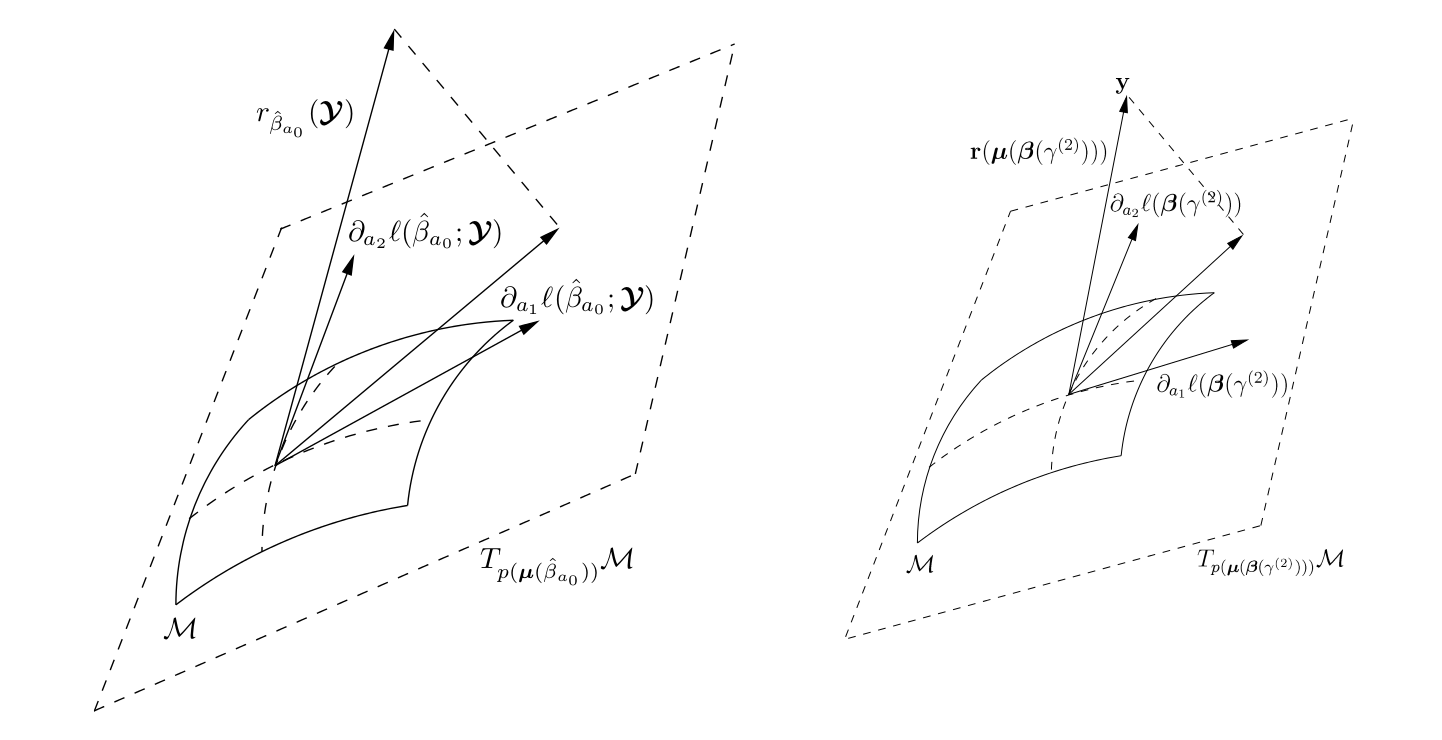
\includegraphics[scale=0.4]{Pictures/diff.png}
%\caption{jo $x$}
\caption{Differential geometrical description of the model extension method for birth-death speciation model with two covariates; in the left side the first predictor $\mathcal{X}_{a_1}$ is found and included in the active set; in the right side the generalized equiangularity condition \ref{le} is satisfied for $\mathcal{X}_{a_1}$ and $\mathcal{X}_{a_2}$ \cite{augugliaro2013differential}}
\label{dglars} 
\end{figure}



 